
\begin{figure}[ht]
\caption{Clustering for 3 variables with 3 silos - (A) categorical variables with  proportion with K-Means and (B)  Categorical with K-modes  }\label{fig:interest} 
  \subcaptionbox*{(A)}[.44\linewidth]{%
    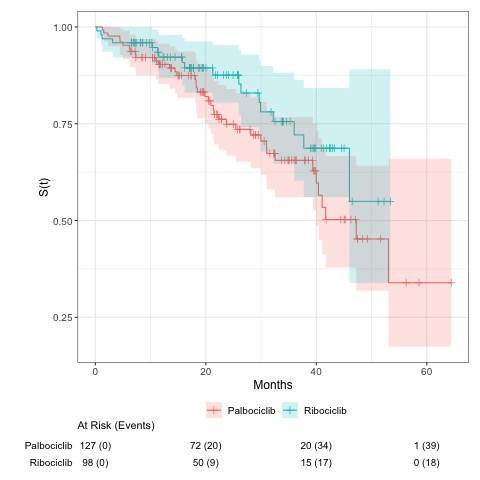
\includegraphics[width=\linewidth]{figures/interest_curve_OS.jpeg}%
  }%
  \hfill
  \subcaptionbox*{(B)}[.44\linewidth]{%
    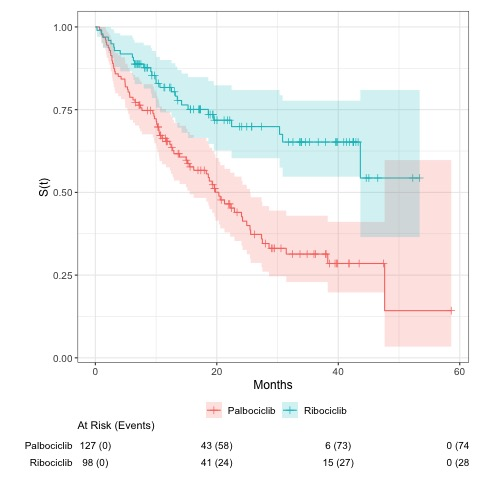
\includegraphics[width=\linewidth]{figures/interest_curve_PFS.jpeg}%
  }
\end{figure}


\begin{figure}[ht]
\caption{Clustering for 3 variables with 3 silos - (A) categorical variables with  proportion with K-Means and (B)  Categorical with K-modes  }\label{fig:tables} 
  \subcaptionbox*{(A)}[.44\linewidth]{%
    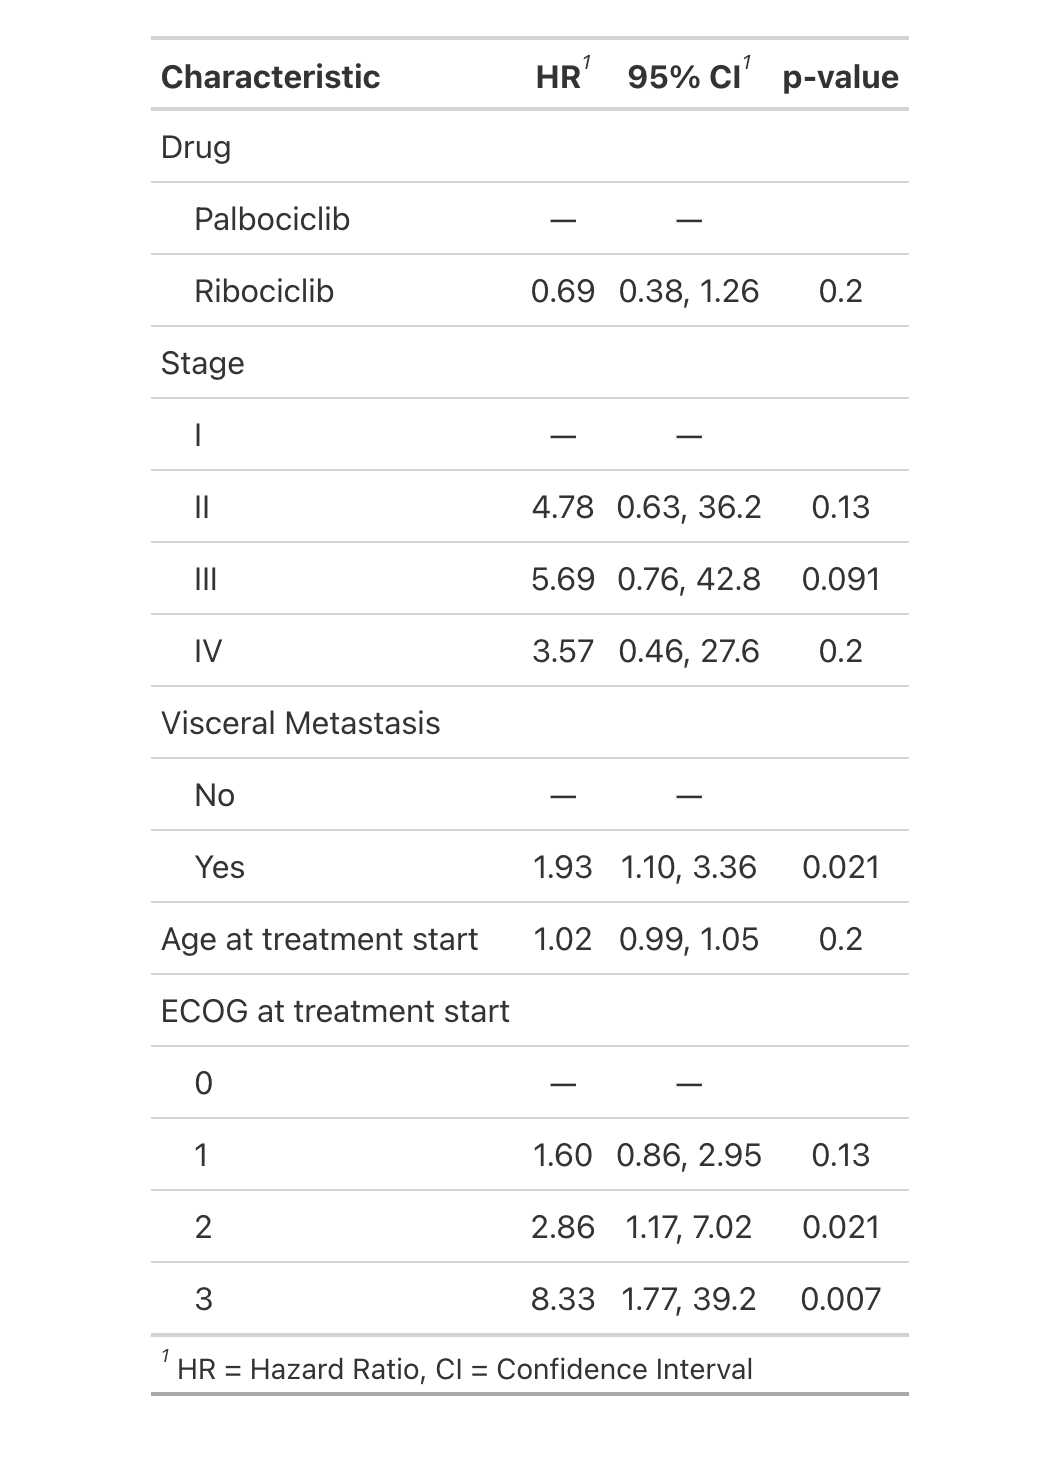
\includegraphics[width=\linewidth]{figures/table_cox_1.jpeg}%
  }%
  \hfill
  \subcaptionbox*{(B)}[.44\linewidth]{%
    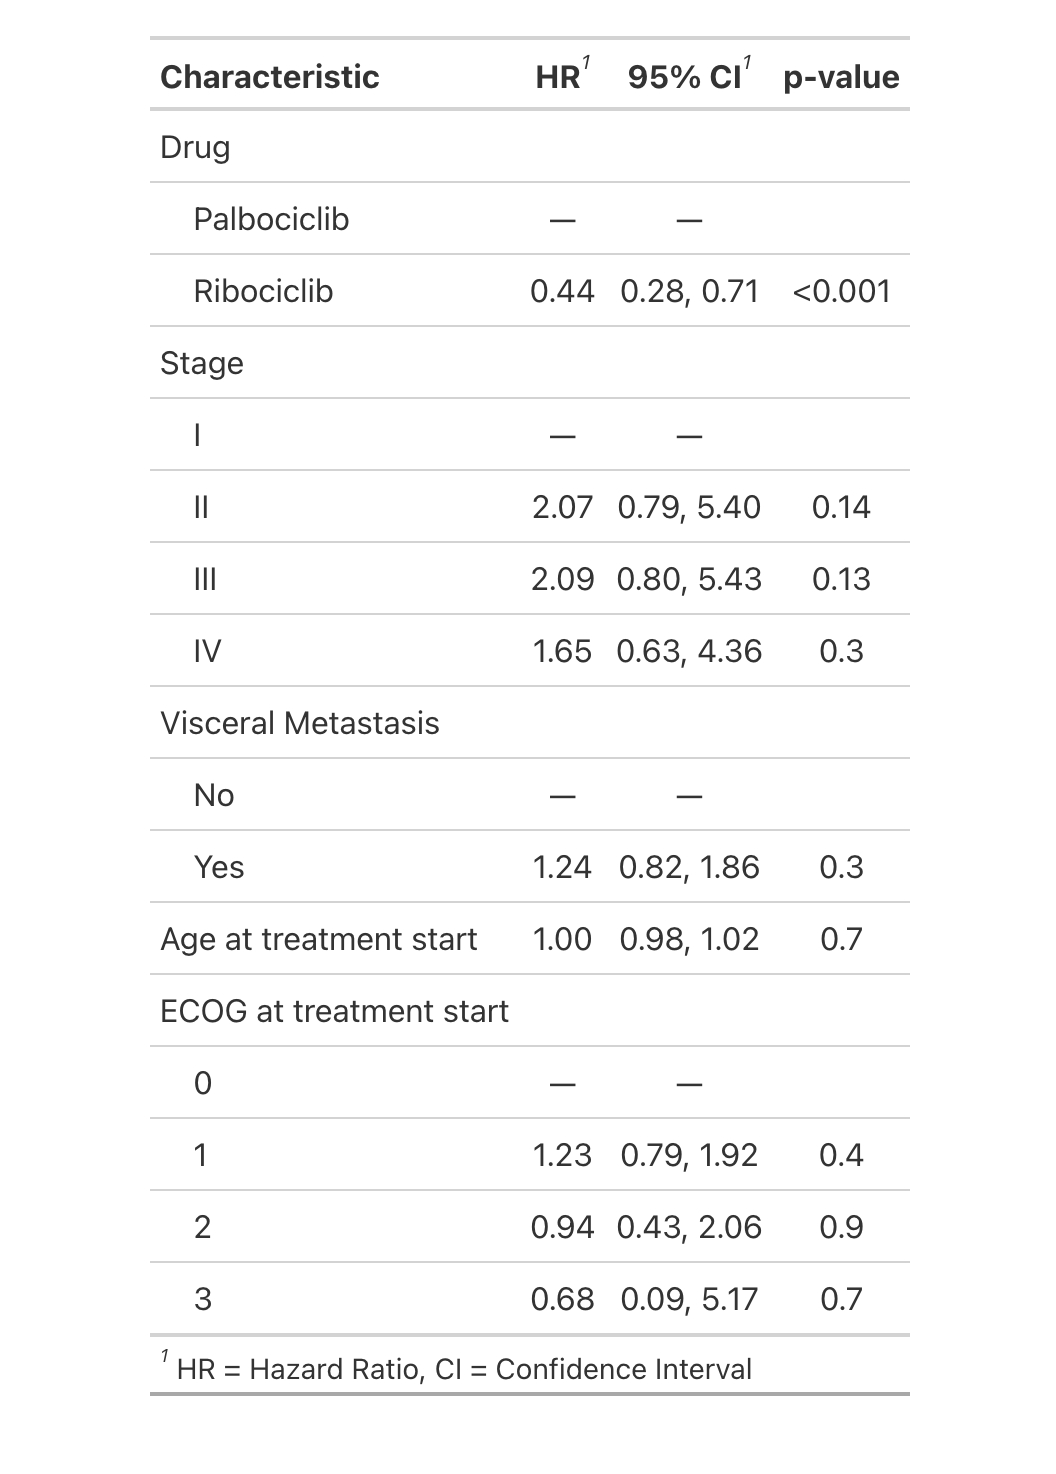
\includegraphics[width=\linewidth]{figures/table_cox_2.jpg.jpeg}%
  }
\end{figure}


\begin{figure}[ht]
\caption{Clustering for 3 variables with 3 silos - (A) categorical variables with  proportion with K-Means and (B)  Categorical with K-modes  }\label{fig:grouped} 
  \subcaptionbox*{(A)}[.44\linewidth]{%
    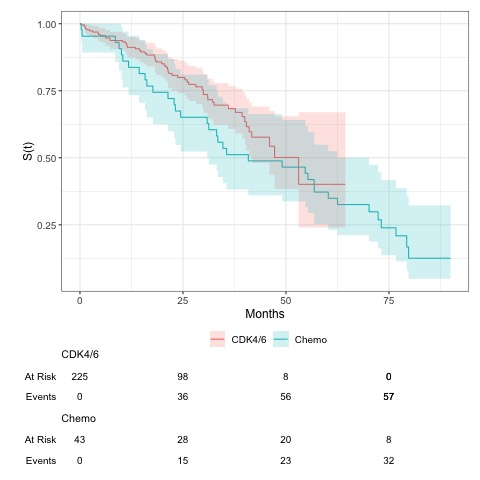
\includegraphics[width=\linewidth]{figures/grouped_curve_OS.jpeg}%
  }%
  \hfill
  \subcaptionbox*{(B)}[.44\linewidth]{%
    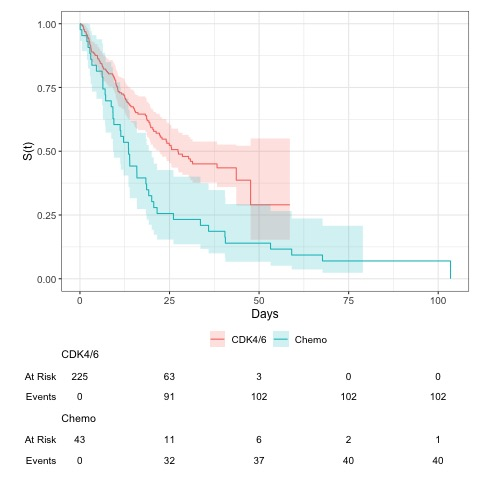
\includegraphics[width=\linewidth]{figures/grouped_curve_PFS.jpeg}%
  }
\end{figure}


\begin{figure}[ht]
\caption{Clustering for 3 variables with 3 silos - (A) categorical variables with  proportion with K-Means and (B)  Categorical with K-modes  }\label{fig:prop_score} 
  \subcaptionbox*{(A)}[.44\linewidth]{%
    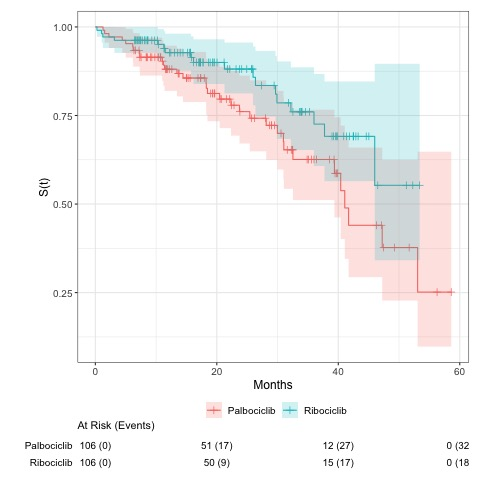
\includegraphics[width=\linewidth]{figures/propensity_score_os.jpg}%
  }%
  \hfill
  \subcaptionbox*{(B)}[.44\linewidth]{%
    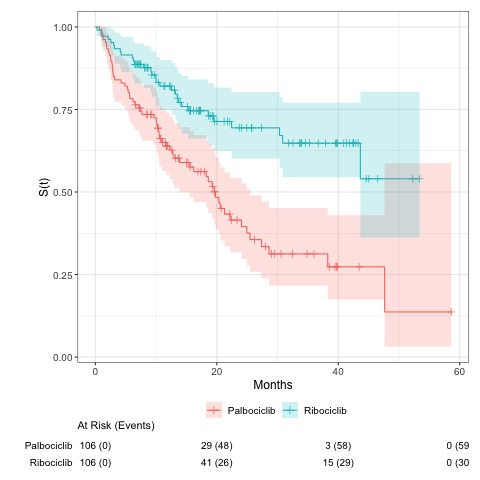
\includegraphics[width=\linewidth]{figures/propensity_score_pfs.jpg}%
  }
\end{figure}


